\documentclass[12pt,a4paper]{article}

\frenchspacing
\setlength\parindent{0pt}

%%%%%%%%%%%%%%%%%%%%%%%%%%%%%%%%%%%%%%%%%%%%%%%%%%%%%%%%%%%%%%%%%%%%%%%%
\usepackage{lmodern}
\usepackage[a4paper,hdivide={30mm,*,30mm},vdivide={30mm,*,30mm}]{geometry}
\usepackage{graphicx}
\usepackage{amsthm}
\usepackage{amsmath}
\usepackage{dsfont}
\usepackage[authoryear,round]{natbib}
\usepackage{iasbib}
\usepackage{subfigure}

\graphicspath{{img/}}

%%%%%%%%%%%%%%%%%%%%%%%%%%%%%%%%%%%%%%%%%%%%%%%%%%%%%%%%%%%%%%%%%%%%%%%%
% Custom Commands
\newcommand{\lsym}{\textit}
\newtheorem{mydef}{Definition}
\DeclareMathOperator*{\argmax}{\text{arg\,max}}
\newcommand{\impl}{\rightarrow}

%%%%%%%%%%%%%%%%%%%%%%%%%%%%%%%%%%%%%%%%%%%%%%%%%%%%%%%%%%%%%%%%%%%%%%%%
% Document Parameters
\title{\textbf{Probabilistic Robot Action Cores\\-- A Roadmap}\\\vspace{.5cm} {\Large Technical Report}}
\author{Daniel Nyga}
\date{\today}

%%%%%%%%%%%%%%%%%%%%%%%%%%%%%%%%%%%%%%%%%%%%%%%%%%%%%%%%%%%%%%%%%%%%%%%%
\begin{document}

\maketitle	

\begin{abstract}
In this report we address the problem of modeling probabilistic dependencies among
concepts in class taxonomies. 
\end{abstract}

\section{Outline}

\begin{enumerate}
	\item Probabilistic Models of Class Hierarchies with Markov Logic Networks.
	\item Learning Sequential Qualitative Prepresentations of Actions from Interactive Computer Games
	\item Incremental Learning of Markov Logic Networks
	\item Active Learning of PRAC Models using Uncertainty Verbalization
	\item Optimization of MLN implementation
\end{enumerate}

\section{Introduction}

Issues addressed in this Technical Report, taken from \cite{nyga12actioncore}:
\begin{enumerate}
    \item \textit{Disambiguation}: naturalistic action 
    specifications exhibit a high degree of ambiguity. As an 
    example, consider the instruction ``Flip!'', which could 
    have several different meanings. Given contextual information, 
    however, e.g. the objects
	\begin{center}
	    \begin{tabular}{l}		
		\lsym{isa}(\lsym{p}, \lsym{Pancake}),
		\lsym{isa}(\lsym{s}, \lsym{Spatula}),
		\lsym{isa}(\lsym{o}, \lsym{Oven}),
	    \end{tabular}
	\end{center}
    a KB modeling action parameterization can be employed to infer 
    what has to be done to which object, based on the ``typical'' 
    meaning and role of the entities $p$, $s$ and $o$. In our example, an appropriate 
    role association would be given by
	
    \begin{center}
	    \begin{tabular}{ll}
		 & $ \lsym{hasRole}_{\lsym{\footnotesize Turn\_around}}(\lsym{p}, \lsym{Theme})$,\\
		 & $ \lsym{hasRole}_{\lsym{\footnotesize Turn\_around}}(\lsym{s}, \lsym{Instrument})$\\
		 and & $ \lsym{hasRole}_{\lsym{\footnotesize Turn\_around}}(\lsym{o}, \lsym{FixedLocation})$.
	    \end{tabular}
	\end{center}
	
    \item \textit{Completion of actions}: naturalistic action 
    specifications are incomplete. As pointed out above, this 
    results from the common human knowledge about actions, which is 
    so self-evident that no one would state it explicitly. In 
    descriptions of activities written by humans, such as cooking 
    recipes, instructions like ``stir occasionally'' can be found 
    very often. These instructions are characterized by extreme 
    underspecification since they lack any information about the 
    objects involved in the respective action. In our examples, it 
    has to be inferred what needs to be stirred (e.g.\ 
    batter) and which utensil is to be used (e.g.\ a spoon or a 
    mixer), etc.\ 
\end{enumerate}
Building abstract event patterns in a probabilistic 
first-order knowledge base. From a probabilistic 
point of view we can formulate this as \begin{eqnarray} \argmax_{
\mbox{\textit{{\footnotesize neededRoles}}}}P_{\textit {Action}}(
\textit{neededRoles}\,|\,\textit{givenRoles}),\nonumber 
\end{eqnarray} where the given roles also include relations that are 
incorporated by an ontology that models taxonomic (\textit {is-a}, 
in symbols $\sqsubseteq$) or mereological (\textit{part-of}, in 
symbols $\preceq$) knowledge. This allows us to model an action core 
at an appropriate level of abstraction, such that it can be applied 
to a large number of real-world scenarios of the same type.

Including a taxonomy of the word senses has several desirable advantages:

\paragraph{Density estimation on nominal data.}The most outstanding 
advantage of including a class taxonomy in a model is that it 
enables to model density functions on categorial data. Usually, when 
dealing with such data, the absence of a total ordering on distinct 
values of a discrete, nonnumeric random variable constrains 
statistical analysis to very basic methods such as histogram-based 
methods. The taxonomic relation, however, induces an ordering on 
values of a categorical domain and thus allows to ``interpolate'' 
between two concepts. As we will show in this work, being aware of a 
class hierarchy underlying a particular domain even allows to 
compute the \emph{expected behavior} of an unknown class, which is 
superior to the commonly used \emph{mode} of a categorial variable. 

\paragraph{Better generalization performance.} Being aware of 
superclass relationships among different classes allows abstracting away
from concrete training examples to more general models

 Given a couple of concrete single action specifications such as 
\begin{center} ``Fill$_{\textit{Action}}$ milk$_{\textit{Theme}}$ 
into a bowl$_{\textit{Destination}}$''\\ and ``Fill
$_{\textit{Action}}$ a glass$_{\textit{Destination}}$ with water
$_{\textit{Theme}}$'', \end{center} the taxonomic relationship 
between milk and water on the one hand, and bowl and glass on the 
other hand, enables abstracting away to more generic patterns such 
as \begin{center} ``Fill$_{\textit{Action}}$ a liquid
$_{\textit{Theme}}$ into a container$_{\textit{Destination}}$. 
\end{center}

Given a previously unseen object, let us assume ``juice'', the most 
probable role assignment of that word can be inferred since 
superclasses are taken into account in the model. 

\paragraph{Less training data needed.} As a consequence of the points 
mentioned in the previous paragraph, a model taking into account 
the taxonomic relationships among classes needs less data to be trained
with to perform comparably well, if not even better than a model not
employing the class taxonomy. 


\begin{itemize}
	\item Refer to the \emph{Yale Shooting Problem} by \cite
	{hanks1987nonmonotonic} here as an example for formalisms that 
	are intrinsically consistent, but produce unexpected behavior 
	when being applied to real-world problems. Today, we find ourselves in a 
	very similar situation, if we want to employ Markov Logic to modeling
	real-world problems. \cite{jain11kr} already has pinpointed some subtleties and 
	fallacies one may encounter when dealing with Markov logic networks
	in knowledge engineering.  
\end{itemize}

\subsection{Requirements for a Taxonomoy-aware Probabilistic KB}

In this section we collect some requirements a taxonomy-aware KB
has to fulfill, which are in our opinion desirable.

\paragraph{Support for unknown concepts.} In practice, there is only 
poor chance that a data set from which we want to train a model is 
sufficiently large, such that it exhaustively covers all relevant 
cases. On the contrary, we experience data that are parse and noisy 
and we cannot expect our data at hand to completely cover all 
concepts that are contained in a particular taxonomy. Hence, the KB 
should be able to perform reasonably well on classes that have not been 
seen in the training set.

\paragraph{Preference for known concepts.} Suppose you have heard a 
particular word always in a specific context in your life, always 
referring to the same class concept, say the word ``bank'', 
referring to a financial institute. Now, you are told that the word
``bank'' might also refer to another concept, i.e.\ a piece of furniture,
but you have never seen a piece of furniture in your life. Then, there
is no reason for ever choosing the newly learned concept, except for
evidence renders the familiar concept truly unlikely. A KB therefore
should prefer known concepts to unknown ones, whenever reasonable.

\paragraph{Monotonously increasing probability in concreteness.} 
Probabilities of concepts should monotonically increase in their 
concreteness, i.e.\ their depth in the taxonomy graph.
 
Humans tend to refer to more ``abstract'' concepts for mainly three 
reasons: 

\begin{enumerate}
	\item \textbf{Subsumption.} One reason why humans draw on more 
	abstract terms in their language is that they intend to refer 
	not only one particular entity in the world, but to a collection 
	of things that share one or more sets of attributes. Subsumption 
	allows to make statements over an arbitrarily large set of 
	entities without repeating utterance for each single entity. 
	This concept of \emph{subsumption} allows to state that, for 
	instance, ``meat is perishable'', without being to repeat this 
	statement for the piece of meat in the world.
	
	\item \textbf{Lack of Knowledge.} A reason for using an abstract 
	terminology is the lack of knowledge about specific objects or 
	actions. If a human, for example, has identified some entity in 
	the world be meat, then he would refer to this entity as 
	``meat'', not knowing if it is actually beef, pork or chicken. 
	In this case, the knowledge of the human does not suffice to 
	further distinguish between different kinds of meat and he has 
	no other choice as to refer to the more abstract term. In the 
	most drastic case, we refer to an entity as a ``thing'', if we 
	do not know anything about it. 
	
	\item \textbf{Sufficient Concreteness/discriminability.} If 
	there is no risk of misinterpreting a statement, humans tend to 
	use more abstract terms. Example: In a recipe for making pork 
	roast, it suffices to refer to the pork as ``meat'', for there 
	are no other kinds of meat involved, which could be confused 
	with the pork. However, unlike the two previous points, this one 
	can be thought of ``syntactic laziness'' (or ``syntactic sugar'' 
	of natural language, respectively). When grounding the terms
	to objects in the real-world, the distinction between ``meat''
	and ``pork'' still is indispensible.
	
\end{enumerate}

\paragraph{Corollary:} The more abstract a terminology is, the 
vaguer is its semantics. As a consequence, any reasoning mechanism 
should prefer more concrete concepts to more abstract ones to be as 
precise as possible. Hence, we argue that any concept should be at least
as probable as all of its superclasses.

\newcommand{\Cup}{\textit{Cup}}
\newcommand{\Thing}{\textit{Thing}}
\newcommand{\Glass}{\textit{Glass}}
\newcommand{\DrinkingVessel}{\textit{DrinkingVessel}}
\paragraph{Proposition: the closed-world assumption is inappropriate 
in learning from natural language.} In literature about knowledge 
engineering, class hierarchies are mostly defined in terms of the 
subsumption principle reported above. We define a concept as a subset
of all indiviuals that have equal or similar properties, e.g.
$$
	\textit{isa}(\Cup, \Thing), \text{ or }\Cup\subset \Thing,
$$
where \textit{Thing} (alse referred to as $\top$) is the set of all individuals.
A particular individual in turn is an element of the concepts it belongs to, e.g.\ 
$$
	\textit{element}(c_{18}, \Cup), \text{ or } c_{18}\in \Cup.
$$
If we now introduce an additional type of drinking vessels, \Glass,
we can subsume all drinking vessels by introducing a new collection:
\begin{eqnarray}	
	\forall x.\ x\in \Cup\impl x\in\DrinkingVessel,\nonumber\\
	\forall x.\ x\in \Glass\impl x\in\DrinkingVessel,\nonumber
\end{eqnarray}
or
\begin{eqnarray}	
	\forall x.\ x\in \DrinkingVessel\impl x\in\Cup\lor x\in\Glass.\nonumber
\end{eqnarray}
The latter is called a \emph{complete decomposition} of the concept \DrinkingVessel.
A disjoint complete decomposition is called a \emph{partition}.

\section{Markov Logic Networks}

Formally, a Markov logic network $L$ is given by a set of pairs $\langle F_i, w_i \rangle$, where $F_i$ is a formula in first-order
logic and $w_i$ is a real-valued weight \cite{richardson06ml}. For each finite domain of discourse $D$ (set of constants%\footnote{In practice, we
%typically assume a typed set of constants/entities and associate with each predicate a signature that determines the types of entities
%it can be applied to.
%}), % $C$ (which constitutes the domain of discourse), 
), 
an MLN $L$ defines a \emph{ground Markov network} $M_{L,D} = \langle X, G \rangle$ 
as follows:

%\vspace{-1.35ex}

\begin{enumerate}
    \setlength{\itemsep}{-0.5ex}
    \item
		$X$ is an indexed set of Boolean random variables. For each possible grounding of each predicate appearing
        in $L$, we add to $X$ a Boolean variable (ground atom).
		We denote by $\mathcal{X} := \mathds{B}^{|X|}$ the set of possible worlds,possible world
	 	i.e. the set of possible assignments of truth values to the variables in $X$.

		\vspace{1ex}
    \item
		$G$ is an indexed set of weighted ground formulas, i.e. a set of pairs $\langle \hat{F}_j, \hat{w}_j \rangle$, 
		where $\hat{F}_j$ is a ground formula and $\hat{w}_j$ is a real-valued weight.
		For each possible grounding $\hat{F}_j$ of each formula $F_i$ in $L$, we add to $G$ 
		the pair $\langle \hat{F}_j, \hat{w}_j = w_i\rangle$.
		With each such pair, we associate
		a \emph{feature} $\hat{f}_j : \mathcal{X} \rightarrow \{0,1\}$, whose value for $x\in \mathcal{X}$ is 1 if $\hat{F}_j$
		is satisfied in $x$ and 0 otherwise, and
        %$M_{L,D}$ contains one feature for each possible grounding of each formula $F_i$ in $L$. The
        %value of this feature is 1 if the ground formula is true, and 0 otherwise. 
		whose weight is $\hat{w}_j$.
\end{enumerate}
The ground Markov network $M_{L,D}$ specifies a probability distribution over 
the set of possible worlds $\mathcal{X}$ 
as follows,
\begin{equation}
		P(X=x) 
			= \frac{1}{Z}\exp\left(\sum_{i=1}^{|L|} {w}_i {n}_i(x)\right)
			= \frac{1}{Z}\exp\left(\sum_{j=1}^{|G|} \hat{w}_j \hat{f}_j(x)\right) 
\label{eq:mln:world-prob}
\end{equation}
where $Z=\sum_{x'\in\mathcal{X}} \exp\left(\sum_i w_i n_i(x')\right) = \sum_{x'\in\mathcal{X}} \exp\left(\sum_j \hat{w}_j \hat f_j(x')\right)$
is a normalisation constant and $n_i(x)$ denotes the number of true groundings of $F_i$ in $x$.
(Definitions taken from \cite{jain12phd})

%\begin{mydef}
%A Markov Logic Network $\lsym{MLN}$ is a set of $N$ tuples $\left\{\left<w_i,F_i\right>\right\}_{i=1}^{N}$,
%where\\
%\begin{tabular}{ll}
	%$F_i$ & is a formula in first-order logic,\\
	%$w_i\in\mathds{R}$ & is a weight attached to $F_i$
%\end{tabular}
%\end{mydef}
%An MLN $\lsym{MLN}$ defines a \emph{ground Markov random field} $M_{\lsym{MLN},D}=\left<X,G\right>$

\section{Word Sense Disambiguation}

We consider the following classification task. Suppose we wish to 
learn a model for the problem of semantic role labeling, which is a 
common task in the field fo natural-language processing. To this 
end, we not only want to consider the single words occuring in a 
natural-language sentence, but also take their super-classes into 
account, which might be obtained by some upper ontology. 

The ontology considered in this work comprises the class concepts 
shown in Figure \ref{fig:taxonomy}. In the remainder of this work, we 
use the terms ``(word) sense'', ``class'' and ``concept'' equivalently.

\begin{figure}[tbp]
	\centering
	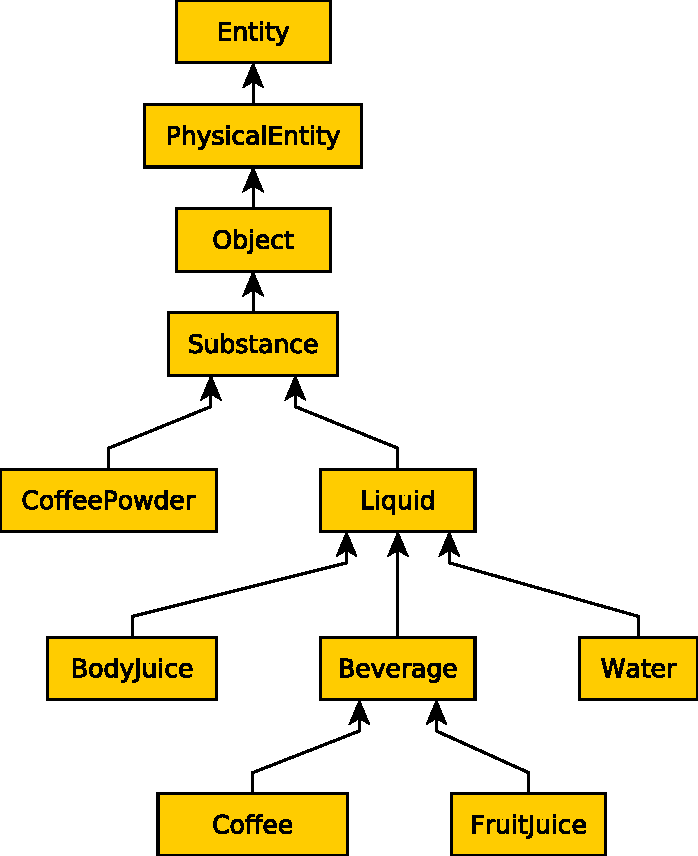
\includegraphics[height=.3\paperheight]{simple_onto.pdf}
	\caption{Class taxonomy used in our example.}
	\label{fig:taxonomy}
\end{figure}

\newcommand{\hasSense}{\textit{hasSense\,}}
\newcommand{\hasRole}{\textit{hasRole\,}}
\newcommand{\Theme}{\textit{Theme}}
\newcommand{\FruitJuice}{\textit{FruitJuice}}
\newcommand{\Beverage}{\textit{Beverage}}
\newcommand{\Liquid}{\textit{Liquid}}
\newcommand{\Substance}{\textit{Substance}}
\newcommand{\PhysicalEntity}{\textit{PhysicalEntity}}
\newcommand{\Entity}{\textit{Entity}}
\newcommand{\isa}{\textit{isa\,}}
\newcommand{\Goal}{\textit{Goal}}
\newcommand{\Water}{\textit{Water}}
\newcommand{\BodyJuice}{\textit{BodyJuice}}
\newcommand{\Coffee}{\textit{Coffee}}
\newcommand{\CoffeePowder}{\textit{CoffeePowder}}

Predicate declarations:
\begin{eqnarray}
	%\hasSense()
	\hasSense(\lsym{word},\lsym{senseID}!,\lsym{sentence})\\
	\isa(\lsym{senseID},\lsym{class})\\
	\hasRole(\lsym{word},\lsym{role}!,\lsym{sentence})
\end{eqnarray}

\noindent Formulas:
\begin{eqnarray}
	0 & & \forall \lsym{w$_1$},\lsym{s$_1$},s,c,r.\ \hasSense(\lsym{w$_1$},\lsym{s$_1$},\lsym{s})\wedge\isa(\lsym{s$_1$},+\lsym{c})\wedge\hasRole(\lsym{w$_1$},+\lsym{r},\lsym{s})
\end{eqnarray}
\\

\begin{tabular}{lll}
	\textbf{Database 1:}														& \textbf{Database 2:}														& \textbf{Database 3:} \\
	$\hasSense(W_1, \lsym{Sense$_1$}, \lsym{S})$		&	$\hasSense(W_1, \lsym{Sense$_1$}, \lsym{S})$		&	$\hasSense(W_1, \lsym{Sense$_1$}, \lsym{S})$			\\
	$\hasRole(W_1, \Theme, \lsym{S})$	&	$\hasRole(W_1, \Theme, \lsym{S})$	&	$\hasRole(W_1, \Theme, \lsym{S})$		\\
	$\isa(\lsym{Sense$_1$}, \FruitJuice)$		&	$\isa(\lsym{Sense$_1$}, \Water)$			&	$\isa(\lsym{Sense$_1$}, \Water)$				\\
	$\isa(\lsym{Sense$_1$}, \Beverage)$			&	$\isa(\lsym{Sense$_1$}, \Liquid)$			&	$\isa(\lsym{Sense$_1$}, \Liquid)$				\\
	$\isa(\lsym{Sense$_1$}, \Liquid)$			&	$\isa(\lsym{Sense$_1$}, \Substance)$		&	$\isa(\lsym{Sense$_1$}, \Substance)$			\\
	$\isa(\lsym{Sense$_1$}, \Substance)$		&	$\isa(\lsym{Sense$_1$}, \PhysicalEntity)$	&	$\isa(\lsym{Sense$_1$}, \PhysicalEntity)$		\\	
	$\isa(\lsym{Sense$_1$}, \PhysicalEntity)$	&	$\isa(\lsym{Sense$_1$}, \Entity)$			&	$\isa(\lsym{Sense$_1$}, \Entity)$ 				\\
	$\isa(\lsym{Sense$_1$}, \Entity)$
\end{tabular}

\vspace{2ex}
We use Pseudo-Log-Likelihood-Learning for obtaining the model parameters.
Learning with the above three databases yields the following MLN:

\vspace{2ex}
\begin{tabular}{ll}
	14.253938 & $\forall \lsym{w$_1$},\lsym{s$_1$},s.\ \hasSense(\lsym{w$_1$}, \lsym{s$_1$}, \lsym{s}) \wedge \isa(\lsym{s$_1$}, \PhysicalEntity) \wedge \hasRole(\lsym{w$_1$}, \Theme, \lsym{s})$ \\
	14.253938 & $\forall \lsym{w$_1$},\lsym{s$_1$},s.\ \hasSense(\lsym{w$_1$}, \lsym{s$_1$}, \lsym{s}) \wedge \isa(\lsym{s$_1$}, \Substance) \wedge \hasRole(\lsym{w$_1$}, \Theme, \lsym{s})$\\
	14.253938 &  $\forall \lsym{w$_1$},\lsym{s$_1$},s.\ \hasSense(\lsym{w$_1$}, \lsym{s$_1$}, \lsym{s}) \wedge \isa(\lsym{s$_1$}, \Liquid) \wedge \hasRole(\lsym{w$_1$}, \Theme, \lsym{s})$\\
	14.253938 & $\forall \lsym{w$_1$},\lsym{s$_1$},s.\ \hasSense(\lsym{w$_1$}, \lsym{s$_1$}, \lsym{s}) \wedge \isa(\lsym{s$_1$}, \Entity) \wedge \hasRole(\lsym{w$_1$}, \Theme, \lsym{s})$\\
	0.693142 & $\forall \lsym{w$_1$},\lsym{s$_1$},s.\ \hasSense(\lsym{w$_1$}, \lsym{s$_1$}, \lsym{s}) \wedge \isa(\lsym{s$_1$}, \Water) \wedge \hasRole(\lsym{w$_1$}, \Theme, \lsym{s})$\\
	-0.693142 & $\forall \lsym{w$_1$},\lsym{s$_1$},s.\ \hasSense(\lsym{w$_1$}, \lsym{s$_1$}, \lsym{s}) \wedge \isa(\lsym{s$_1$}, \Beverage) \wedge \hasRole(\lsym{w$_1$}, \Theme, \lsym{s})$\\
	-0.693142 & $\forall \lsym{w$_1$},\lsym{s$_1$},s.\ \hasSense(\lsym{w$_1$}, \lsym{s$_1$}, \lsym{s}) \wedge \isa(\lsym{s$_1$}, \FruitJuice) \wedge \hasRole(\lsym{w$_1$}, \Theme, \lsym{s})$
\end{tabular}

\section{Inference for Word Sense Disambiguation}

In this section analyze the behavior of our learned models when 
being applied to the problem of Word Sense Disambiguation and 
pinpoint some issues that might cause unexpected behavior.

Having trained the original MLN with databases 1-3, we seek to use 
the model in order to resolve word sense ambiguities that we might 
encounter in analyzing natural-language texts. Given a word in 
natural language, the WordNet lexical database can be employed to 
obtain a set of different meanings of that word. For the word 
``coffee'', for example, WordNet returns two different class 
concepts this word might refer to (among others), namely 
$\lsym{Coffee}$  and $\lsym{CoffeePowder}$. However, in our small 
example, we restrict ourselves to these two possible senses.

Let $M_{L,D} = \langle X, G \rangle$ be the ground Markov random 
field defined by $M$ as above. Let $S=(W_1, \ldots,W_n)$ be the 
natural-language sentence under consideration, consisting of $n$ 
words $W_i$, and let $\Sigma(w_i)$ be the set of possible word 
senses for the $i$-th word. We then add to the set 
$G=\langle\widehat{F}_i, \widehat{w}_i\rangle$ of ground formulas 
one disjunction of possible word senses for each word, which we 
assign an infinite weight (i.e.\ a hard constraint):

\begin{eqnarray}
	G' = G\cup\bigcup_{w\in S}\left\{\left<\infty,\bigvee_{s\in\Sigma(w)}\hasSense(w,s,S)\right>\right\}\label{eq:sensedisjunction}
	%\lsym{MLN}\,' = &\left\{\left<w_i,F_i\right>\right\}_{i=1}^N&\cup\bigcup_{w\in S}\left\{\left<\infty,\bigvee_{s\in\Sigma(w)}\lsym{hasSense}(w,s,S)\right>\right\}
\end{eqnarray}

MPE Inference:
\begin{eqnarray}
	\argmax_{x\in\mathcal{X}}P\left(x\left|\,\widehat{F}_e,M_{L,D}\right.\right),\label{eq:mpe-inference}
\end{eqnarray}

where $\widehat{F}_e$ is a set of ground literals representing the 
observed evidence given by the class hierarchy (i.e.\ the \textit
{isa}, in symbols $\sqsubseteq$) relation, which is treated as a 
closed-world predicate (i.e. we assume falsity for all atoms not 
given by the class taxonomy):

\begin{eqnarray}
	\widehat{F}_e=\bigcup_{c\in\top}\bigcup_{s\sqsubseteq c}\{\textit{isa}(s,c)\}
\end{eqnarray}
 
\subsection{Problem Formulation}

Core problem: Treatment of unknown senses, i.e.\ senses that have 
not been seen in the training data. We can differentiate two cases. 

\paragraph{At least one sense is known.} The word is contained in 
the training data, so at least one possible sense of that word is 
contained in the model. If, for instance, we have encountered the 
word ``milk'' in the sense \FruitJuice\ exclusively in our training 
data, this sense is part of the model and occurs in at least one 
formula.
 
Suppose we now are to associate a sense to the word $W=$ ``juice'', 
we would expect our model to assign precisely that sense to this 
word. According to (\ref{eq:sensedisjunction}), we take into account 
all possible word senses and add to our model the ground disjunction

\begin{eqnarray}
	\left<\infty, \hasSense(W, \FruitJuice, S)\vee \hasSense(W, \BodyJuice, S)\right>\nonumber
\end{eqnarray}

with infinite weight, specifying that $W$ necessarily needs to be 
assigned exactly one of that senses in every consistent world. 
However, as we will show in the following, this results in undesired 
behavior, making the model always assigning the sense \BodyJuice\ to 
$W$. Introducing a new concept \BodyJuice\ in the domain of possible 
word senses implicitly introduces the formula

\begin{eqnarray}
	0 & &\forall w_1,s_1,s.\ \hasSense(w_1,s_1,s)\wedge\isa(w_1,BodyJuice),\nonumber
\end{eqnarray}

with zero weight. Assuming that, in our ontology, the word ``juice'' 
can only have these two meanings, there are two possible worlds with 
probability larger than 0. According to (\ref{eq:mln:world-prob}), 
the probability of the world $x$ in which $\hasSense(W,\BodyJuice,S)$
is true is

\begin{eqnarray}
	P(x_{\models\hasSense(W,\BodyJuice,S)})=\alpha\cdot\exp (4\cdot 14.253938), \nonumber
\end{eqnarray} 
 
whereas the world in which  $\hasSense(W,\FruitJuice,S)$ is true has probability 
 
\begin{eqnarray}
	P(x_{\models\hasSense(W,\FruitJuice,S)})=\alpha\cdot\exp (4\cdot 14.253938 - 2\cdot 0.693142),\nonumber
\end{eqnarray}

such that MPE inference according to (\ref{eq:mpe-inference}) would 
yield \BodyJuice\ as the most probable sense assignment for the word 
``juice''. This seems counterintuitive, since the \FruitJuice\ 
concept occurs in the training data, hence is part of the model and 
we intuitively would expect the model to remember this concept 
taking the role \Theme.

\paragraph{All senses are unknown.} In case we encounter a word that 
we have not seen in the training data, it is likely that none of the 
possible senses of that word is part of the model. As an example, 
consider the word ``coffee'' with the two possible word senses 
above, namely \Coffee\ and \CoffeePowder. In this case, adding the 
ground formula

\begin{eqnarray}
	\left<\infty, \hasSense(W, \Coffee, S)\vee \hasSense(W, \CoffeePowder, S)\right>\nonumber	
\end{eqnarray}

yields two possible worlds $x_{\models\hasSense(W,\Coffee,S)}$ and
$x_{\models\hasSense(W,\CoffeePowder,S)}$ with probabilities

\begin{eqnarray}
	&& 	P(x_{\models\hasSense(W,\CoffeePowder,S)})=\alpha\cdot\exp (4\cdot 14.253938), \nonumber\\
	\text{and}&& P(x_{\models\hasSense(W,\Coffee,S)})=\alpha\cdot\exp (4\cdot 14.253938 - 0.693142),\nonumber
\end{eqnarray}

since only those concepts are taken into account, which are contained in
both the taxonomic path and the MLN model. 

This results from the negative weights of formulas correlating the 
concepts \FruitJuice\ and \Beverage, respectively, which indicate 
that any world, in which the sense \Beverage\ is selected is half as 
probable as a world, in which the sense \Liquid\ holds (as long as 
no other formulas hold). 

\subsection{Approach: Elimination of Negative Weights}

Somehow engineer weights, such that worlds with known senses always gain 
higher probability than worlds with unknown senses:
\begin{eqnarray}
	\forall x. \textit{containsUnknownSenses(}
\end{eqnarray} 

\subsection{Approach: Include Inapplicable Senses into the Model}

For each sense contained in the training data, add \emph{all} siblings
of that concept to the domain of possible senses:
\begin{eqnarray}
	\textit{dom}(\textit{sense})=\{s\mid s \text{ is a sense in the data}\}\cup\bigcup_{s}\textit{siblings}(s)\nonumber
\end{eqnarray}

This will enforce all senses that have not been seen in the training 
data to get $\approx$0 probability, and senses that have been seen 
$>$0 probability. However, such a model makes strong assumptions 
about concepts not being part of the training data, which is 
undesired.


\subsection{Approach: Similarity-based Weight Combination}

Idea: For any class concept not contained in the model, make it 
behave like similar concepts that are contained in the model. 
Example: Make \Coffee\ behave like \FruitJuice, based on their 
semantic similarity. To this end, we can introduce a new formula for 
the concept \Coffee,

\begin{eqnarray}
	\left<\hat{w},\ \forall w_1,s_1,s.\ \hasSense(w_1,s_1,s)\wedge\isa(w_1,\Coffee) \right> ,\nonumber
\end{eqnarray}
with weight
\begin{eqnarray}
	\hat{w}=\sum_{c\in\top}\text{sim}(\Coffee,c)\cdot w_{f_{c}},\nonumber
\end{eqnarray}

where $w_{f_{c}}$ is the weight of the corresponding MLN formula 
modeling the correlation of the concept $c$ and the role \Theme\ and 
sim$(\Coffee,c)$ is the semantic similarity of the class concept $c$ 
and the concept \Coffee.

\subsection{Approach: Chain Rule Decomposition}

Problem with the joint probability of senses and roles: The joint 
probability of senses and roles of the form $P(S=\widehat{s}\wedge 
R=\widehat{r})$ captures two phenomena:

\begin{enumerate}

	\item The co-occurrence of a particular sense $\widehat{s}$ and 
	a particular role $r$.

	\item The a-priori probability of a word having a particular 
	sense $\widehat{s}$.

\end{enumerate}

$P(S=\widehat{s}\wedge R=\widehat{r})=P(R=\widehat{r}\mid S=\widehat{s})\cdot P(S=\widehat{s})$
 
\section{Yet Another Approach}

\newcommand{\norm}{\textit{Norm}}

Idea: Treat unknown concepts as their most specific known 
superclass(es), where that superclass is to incorporate the behavior 
of its child concepts. This can be accomplished by rendering 
formulas true that contain derived concepts of the same superclass. 
For spatial reasons and in order to keep the notation uncluttered, 
we write single propositions in the form of $X$ and $X\land Y$ in 
the following, which are to be read as ``something is an $X$'' and 
``something is an $X$ and a $Y$'', respectively.

\subsection{Single Inheritance}

In this section we only consider the simple case of single 
inheritance, i.e.\ the class taxonomy represents a partition of the 
concept space, such as the one given by Figure \ref{fig:taxonomy1}.

The goal is to represent a joint probability distribution over the 
taxonomy:

$P(a,b,c,d,e,f)$

Some Observations: 
\begin{itemize}

	\item We need to consider a particular leaf concept as its path 
	from the concept node to the root node, i.e. the probabilty of 
	something being an $F$, $P(F) = P(A, C, F)$, for
	%P(A, C, F, 
	%\lnot B, \lnot D, \lnot E) = $, since 
	$$P(F)=\sum_{(a,b,c,d,e,f)\in\mathds{B}^{6}}P(F,a,b,c,d,e)=P(A,C,F
	,\lnot B,\lnot D,\lnot E)=P(A, C, F),$$ since all of the joint 
	combinations which are inconsistent with the taxonomy graph have 
	zero probability.
	
	\item In case of a concept on a higher level of abstraction, we 
	have to sum over all leaf nodes contained in the subtree of that 
	concept, e.g.\ $$P(B)=P(A,B,D)+P(A,B,E)+P(A,B,\lnot D,\lnot E)$$ 
	Such a concept might also be \emph{neither} of its subclasses, 
	e.g.\ $P(A,B,\lnot D,\lnot E)$ 
	
	\item The joint probability distribution can be factorized 
	according to the taxonomy graph: $$ P(a,b,c,d,e,f)=P(d,e,f\mid 
	b,c)P(b,c\mid a)P(a) $$
    
\end{itemize}

In such a case of single inheritance (Figure \ref{fig:taxonomy1}), the MLN given by
\begin{eqnarray}
	w_{D} & &D\lor (\lnot D\land\lnot E\land B\land\norm_B(D))\lor (\lnot B\land\lnot C\land A\land\norm_A(B)\land\norm_B(D)),\label{eq:f:w_x1}\nonumber\\
	w_{E} & &E\lor (\lnot E\land\lnot D\land B\land\norm_B(E))\lor (\lnot C\land\lnot B\land A\land\norm_A(B)\land\norm_B(E)),\label{eq:f:w_x2}\nonumber\\
	w_{F} & &F\lor (\lnot F\land C\land\norm_C(F))\lor (\lnot C\land\lnot B\land A\land\norm_A(C)\land\norm_C(F))\nonumber
\end{eqnarray}

models the influence of concepts $D$ and $E$ (and $F$, 
respectively), but the formulas are also applicable in case of a 
concept which ``is a $B$'', but neither a $D$ nor an $E$ (or an $F$
). For both formulas being true in such a case, we need a helper 
predicate

\begin{eqnarray}
    &\norm_X(\textit{Subclasses}_X!)\nonumber\\
    &\textit{dom}(\textit{Subclasses}_X)=\{x\mid x\in\textit{children}(X)\}\nonumber
\end{eqnarray}

which ensures that in case of an unkown word only one of the 
formulas can hold. This is important since, if we encounter a 
concept that is not contained in the training data, say $X_3$ in the 
above taxonomy, both formulas would apply in this case resulting in 
a probability $P(x_{x\models X_3})\propto \exp({w_{X_1}+w_{X_2}})$, 
wich overestimates the actual influence of concept $X_3$. Note that 
the influence of any unknown concept would depend on the mere number 
of siblings in the taxonomy in such a model, which is 
counterintuitive. Having modeled the \norm\ predicate as a 
functional constraint, the distribution given by (\ref{eq:f:w_x1}) 
and (\ref {eq:f:w_x2}) models the behavior of $X_3$ as an average of 
$X_1$ and $X_2$. If the prior distributions of $X_1$ and $X_2$ are 
known as well, the distribution models the expectation of any 
unknown concept $X_i\sqsubseteq X$ based on the observed behavior 
and frequencies of its siblings (and/or superclasses).

\subsection{Multiple Inheritance}

\paragraph{Balanced Case.} All paths of a particular concept to the root node have
	the same length. The taxonomy then represents a factorization of 
	the joint distribution $$P(A,B,C,E,F,\lnot G,H)=P(H,\lnot G\mid 
	F,E)P(F,E\mid C,B)P(C,B\mid A)P(A),$$ for $H$, and 
	$$P(A,B,C,E,F,G,\lnot H)=P(G,\lnot H\mid \lnot F,E)P(\lnot 
	F,E\mid C,B)P(C,B\mid A)P(A)$$ for $G$, according to the 
	underlying graph structure.

In the case of multiple Inheritance (with red arrows in Figure \ref{fig:onto} included),
we need to take into account that a particular concept might have multiple
superclasses. We therefore need to adapt the right part of the disjunction
to be applicable to all direct superclasses and to incorporate their behavior:
\begin{eqnarray}
	A(X_2)=\lnot X_2\land (X\lor Y)\land\lnot X_1\land\lnot Y_1\land(\norm_X(X_2)\lor\norm_Y(X_2)),
\end{eqnarray}
which might yield unsound results, since the disjunction $\norm_X(X_2)\lor\norm_Y(X_2)$
would gain much more probability just because of the fact that some concept
has more superclasses than others. This is counterintuitive.

The correct probability we would like our model to represent is the probabilty
of $X_2$ being true, given knowledge about $X$ and $Y$, i.e.\
\begin{eqnarray}
	P(X_2\mid X,Y)P(X,Y) + P(X_2\mid \lnot X,Y)P(\lnot X,Y)+P(X_2\mid X,\lnot Y)P(X,\lnot Y)\nonumber
\end{eqnarray}
In terms of logic, we can model this distribution as
\begin{eqnarray}
	A(X_2)&=&(\lnot X_2\land\lnot X_1\land\lnot Y_1\land X\land Y\land\norm_{X,Y}(X_2))\nonumber\\
	&&\lor (\lnot X_2\land\lnot X_1\land\lnot Y_1\land X\land\lnot Y\land\norm_{X,\lnot Y}(X_2))\nonumber\\
	&&\lor (\lnot X_2\land\lnot X_1\land\lnot Y_1\land\lnot X\land Y\land\norm_{\lnot X,Y}(X_2))\nonumber
\end{eqnarray}

TODO:
\begin{itemize}
    \item There is no well-defined decomposition of the joint distribution
    over all concepts, which corresponds to the graph structure of the taxonomy. 
\end{itemize}

\begin{figure}
	\centering
	\subfigure[Single Inheritance]{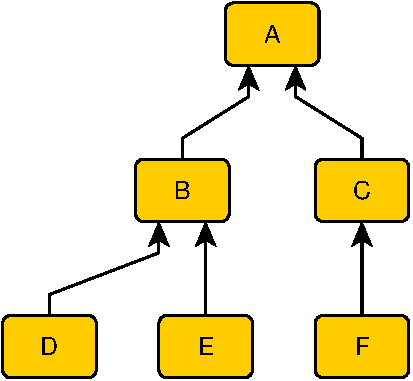
\includegraphics[width=.25\columnwidth]{img/taxonomy1.pdf}\label{fig:taxonomy1}}\hfill
	\subfigure[Multiple Inheritance, balanced]{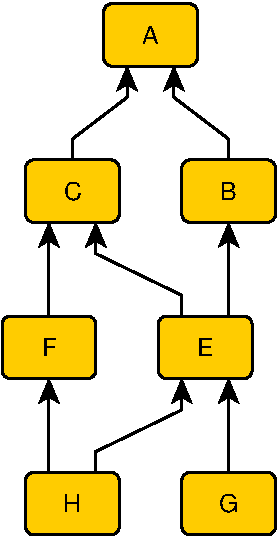
\includegraphics[width=.25\columnwidth]{img/taxonomy2.pdf}\label{fig:taxonomy2}}\hfill
	\subfigure[Multiple Inheritance, imbalanced]{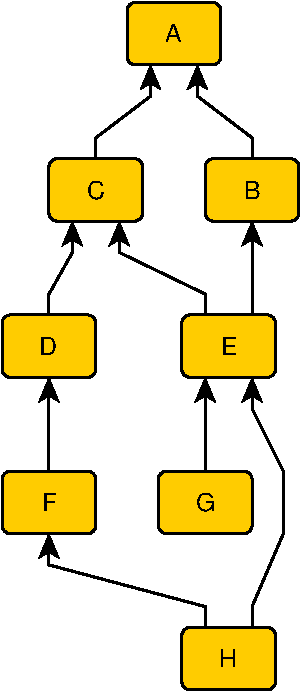
\includegraphics[width=.25\columnwidth]{img/taxonomy3.pdf}\label{fig:taxonomy3}}
    \caption{Three exemplary class taxonomies with increasing complexity.}
	\label{fig:taxonomies}
\end{figure}


%%%%%%%%%%%%%%%%%%%%%%%%%%%%%%%%%%%%%%%%%%%%%%%%%%%%%%%%%%%%%%%%%%%%%%%%		
\bibliographystyle{plainnat}
\allbibliography{literature}

\end{document}
%%%%%%%%%%%%%%%%%%%%%%%%%%%%%%%%%%%%%%%%%%%%%%%%%%%%%%%%%%%%%%%%%%%%%%%%
